\documentclass[../../main.tex]{subfiles}

 \lhead{Implementation: Software}
 
\begin{document}
\lstset{language=Java} 
	\subsection{Software}
		
		%Overall idea
		As a software patch was already in use with the \ac{VSS}, the idea was to extend this software patch to accommodate the newly proposed functionality.

		This section will first give a quick overview of the original max patch and then an overview of the newly produced software with a simple explanation of how it works, followed by a more detailed explanation of how the two main parts of the software work.

		\subsubsection{Software Overview}

			\paragraph{The Original Patch}
			\label{softwareoverview:original}
				The original max patch was used to convolve a real time audio signal with a set of four \ac{RIR}'s simultaneously, allowing the user to turn their head in the \ac{VAE} through the use of an Oculus Rift as a head tracking device. Four positions within the \ac{VAE} were available. To select one, the user (or an operator) selected an `open' button which prompted a file navigation window. The \ac{RIR} files then had to be found (in the correct order) and opened one at a time, with a new file window opening after each file had been selected. Figure~\ref{original} shows this.

				This was the primary aspect of the original patch that needed extending to make the process automatic.

					%-------------Max UI Flow diagram-------------%
				\begin{figure}[H]
					\centerline{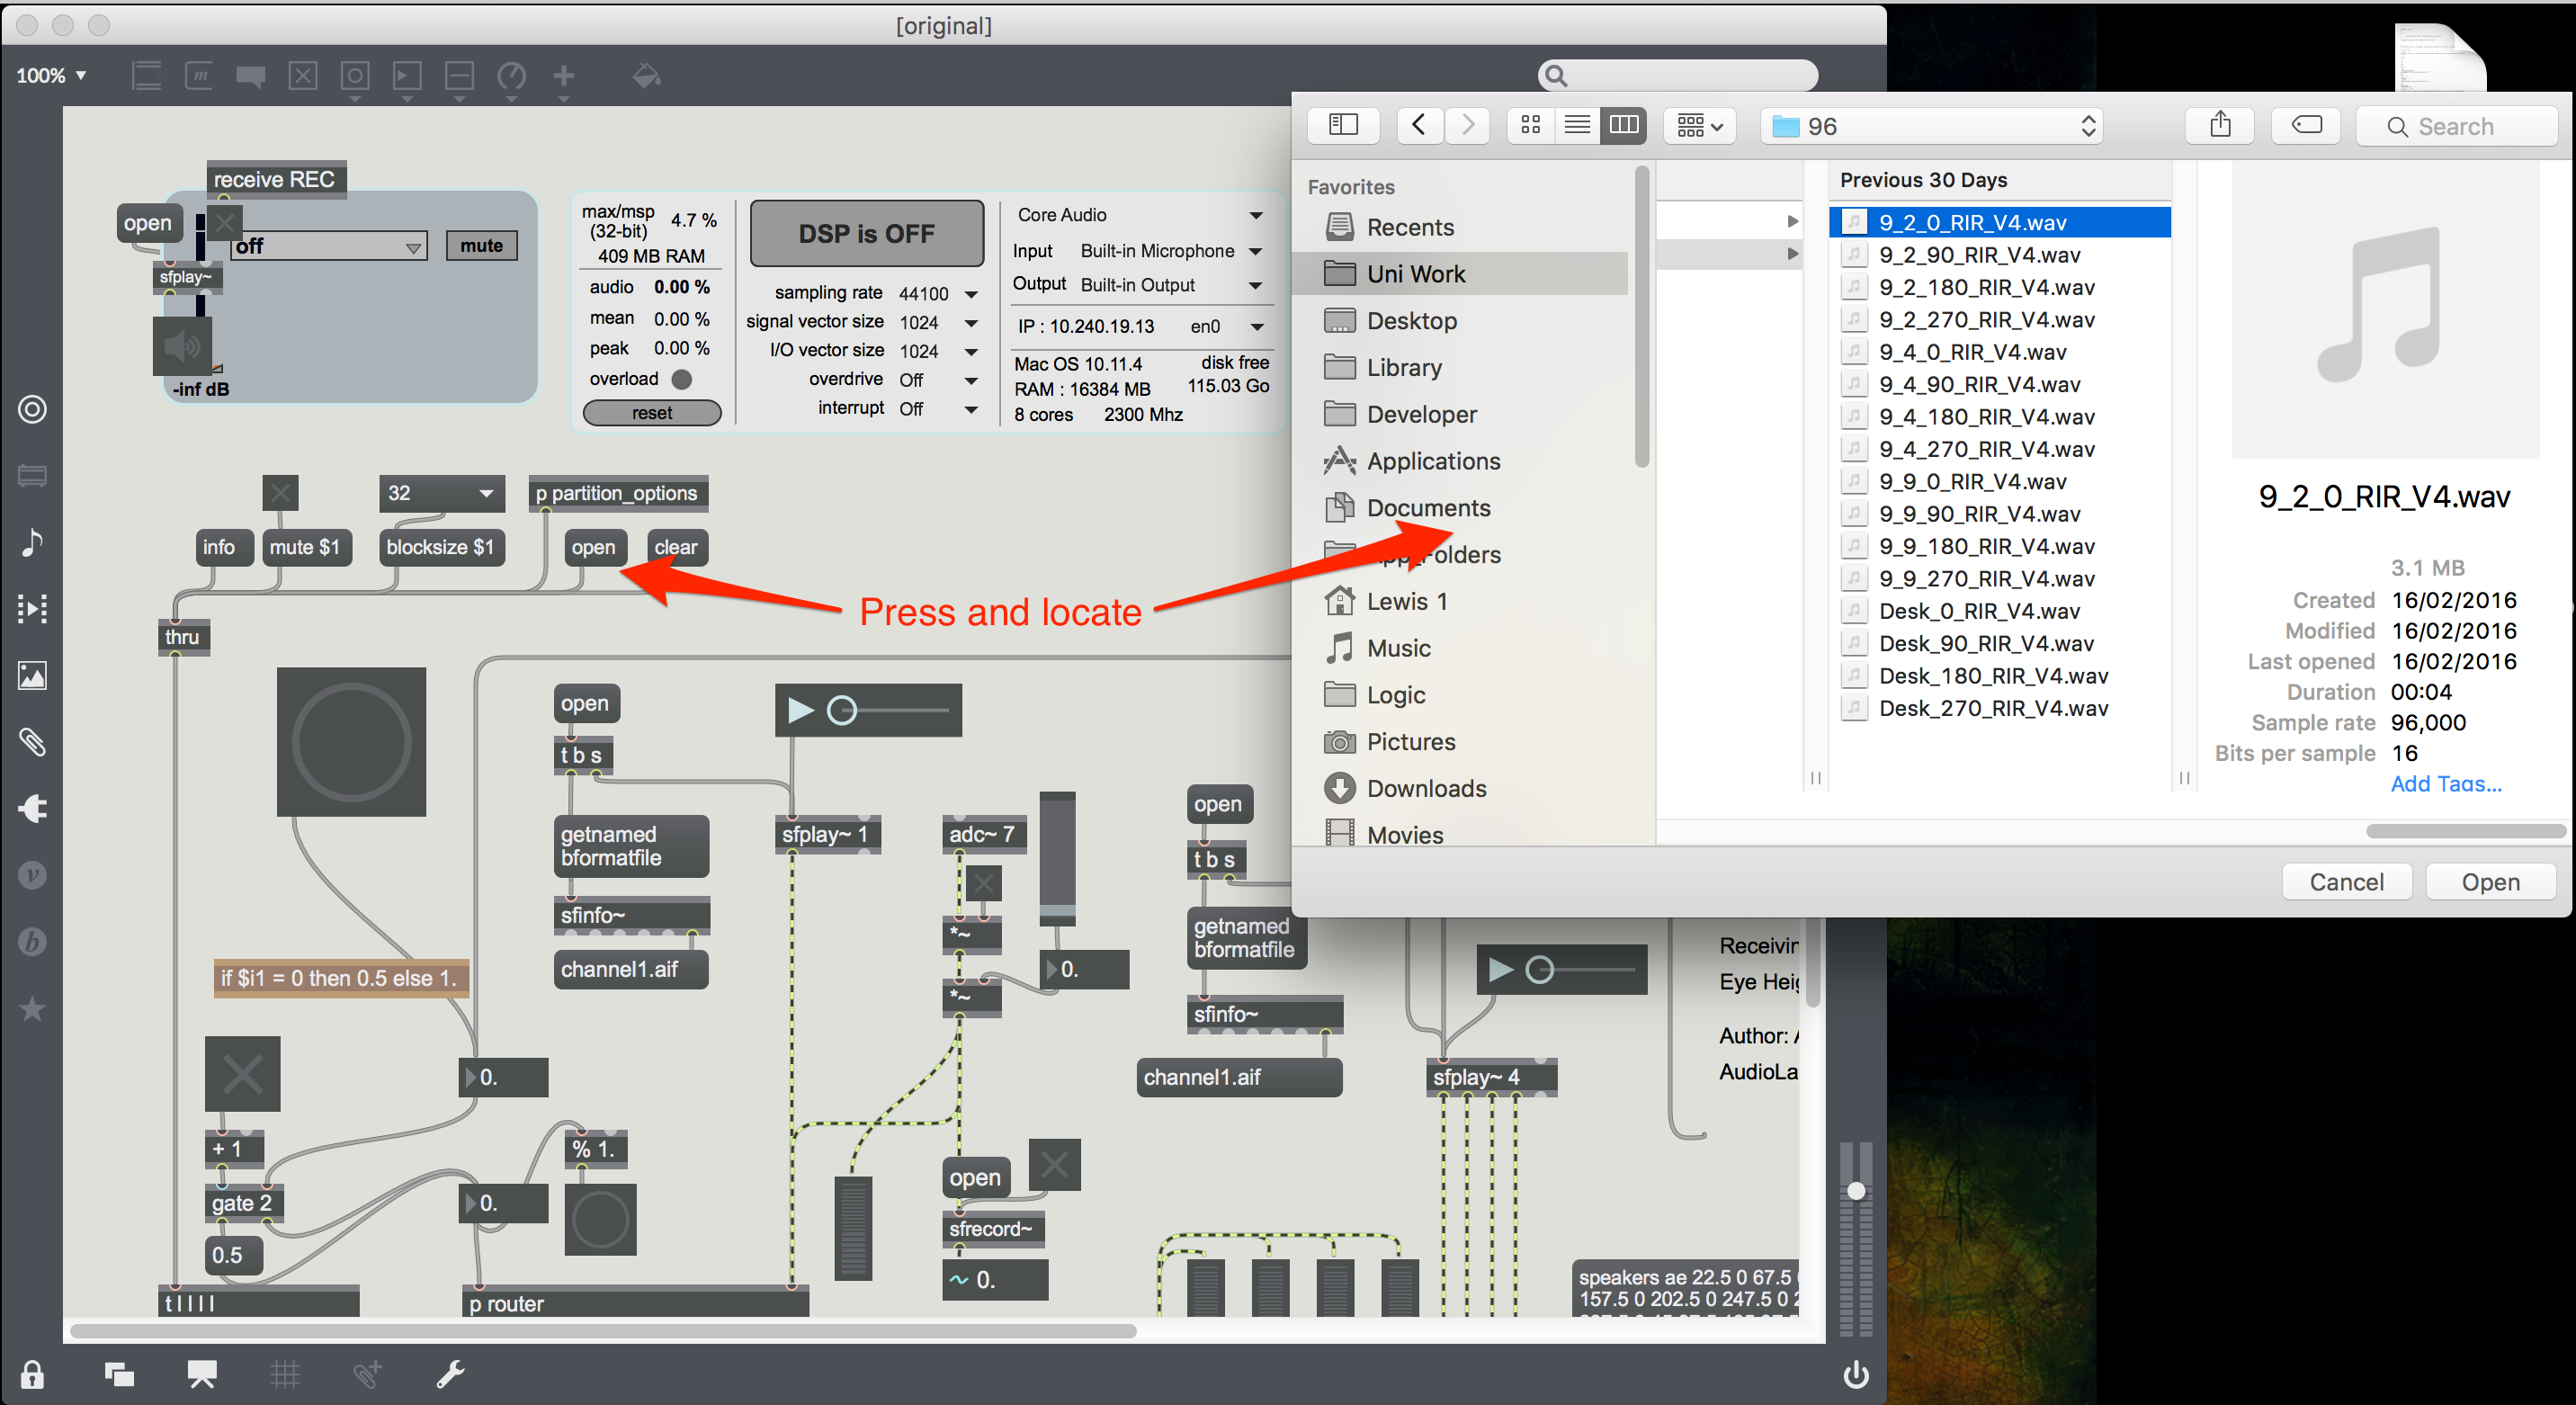
\includegraphics[scale = 0.4]{Sections/Implementation/Max/images/Max/OriginalPatch_Edit.png}}
					\caption{Original Max patch used in the \ac{VSS} showing the file location window that pops up 4 times.}
					\label{original}
				\end{figure}

			\paragraph{Extended Patch Overview}
				Figure~\ref{myPatch} shows an annotated top level view of the Max patch produced to take a user input, load the appropriate \ac{RIR} files and convolve with a real time audio input. The annotated sections can be described as follows:

				\textbf{1:} Two buttons used to reset the system and start the timer used when moving around the space. The settings patch extends to provide a range of options including the density of 

				\textbf{2:} Here, an audio file can be loaded into the system and used instead of a real time audio input. This is used in user test \#3.

				\textbf{3:} A timer used to load new \ac{RIR} files when appropriate.

				\textbf{4.1:} Patches that send a user interface to an iPad which allows a user to select a location within the \ac{VAE}. User interaction is monitored (in the form of screen coordinates) and sent to \textbf{4.2}.

				\textbf{4.2:} Takes the coordinates of the user input and calculates which (if any) \ac{RIR} file should be loaded into the system, in section \textbf{4.3}.

				\textbf{4.3:} Three patches (extended versions of the max explained in section~\nameref{softwareoverview:original}) used to simultaneously convolve an audio signal (real time or audio file) with four directional \ac{RIR} files. While one loads the next necessary \ac{RIR} file the other two are used to simulate the movement of the user by panning the real time audio between the two currently running convolutions. This is how the user is moved along a path, explained in section~\nameref{iteration3}.

				\textbf{5:} An extended version of the real time head-tracking system used in the original patch, used to pan between the four directional \ac{RIR}'s to simulate head movement in the \ac{VAE}.

				%-------------Max UI Flow diagram-------------%
				\begin{figure}[H]
					\centerline{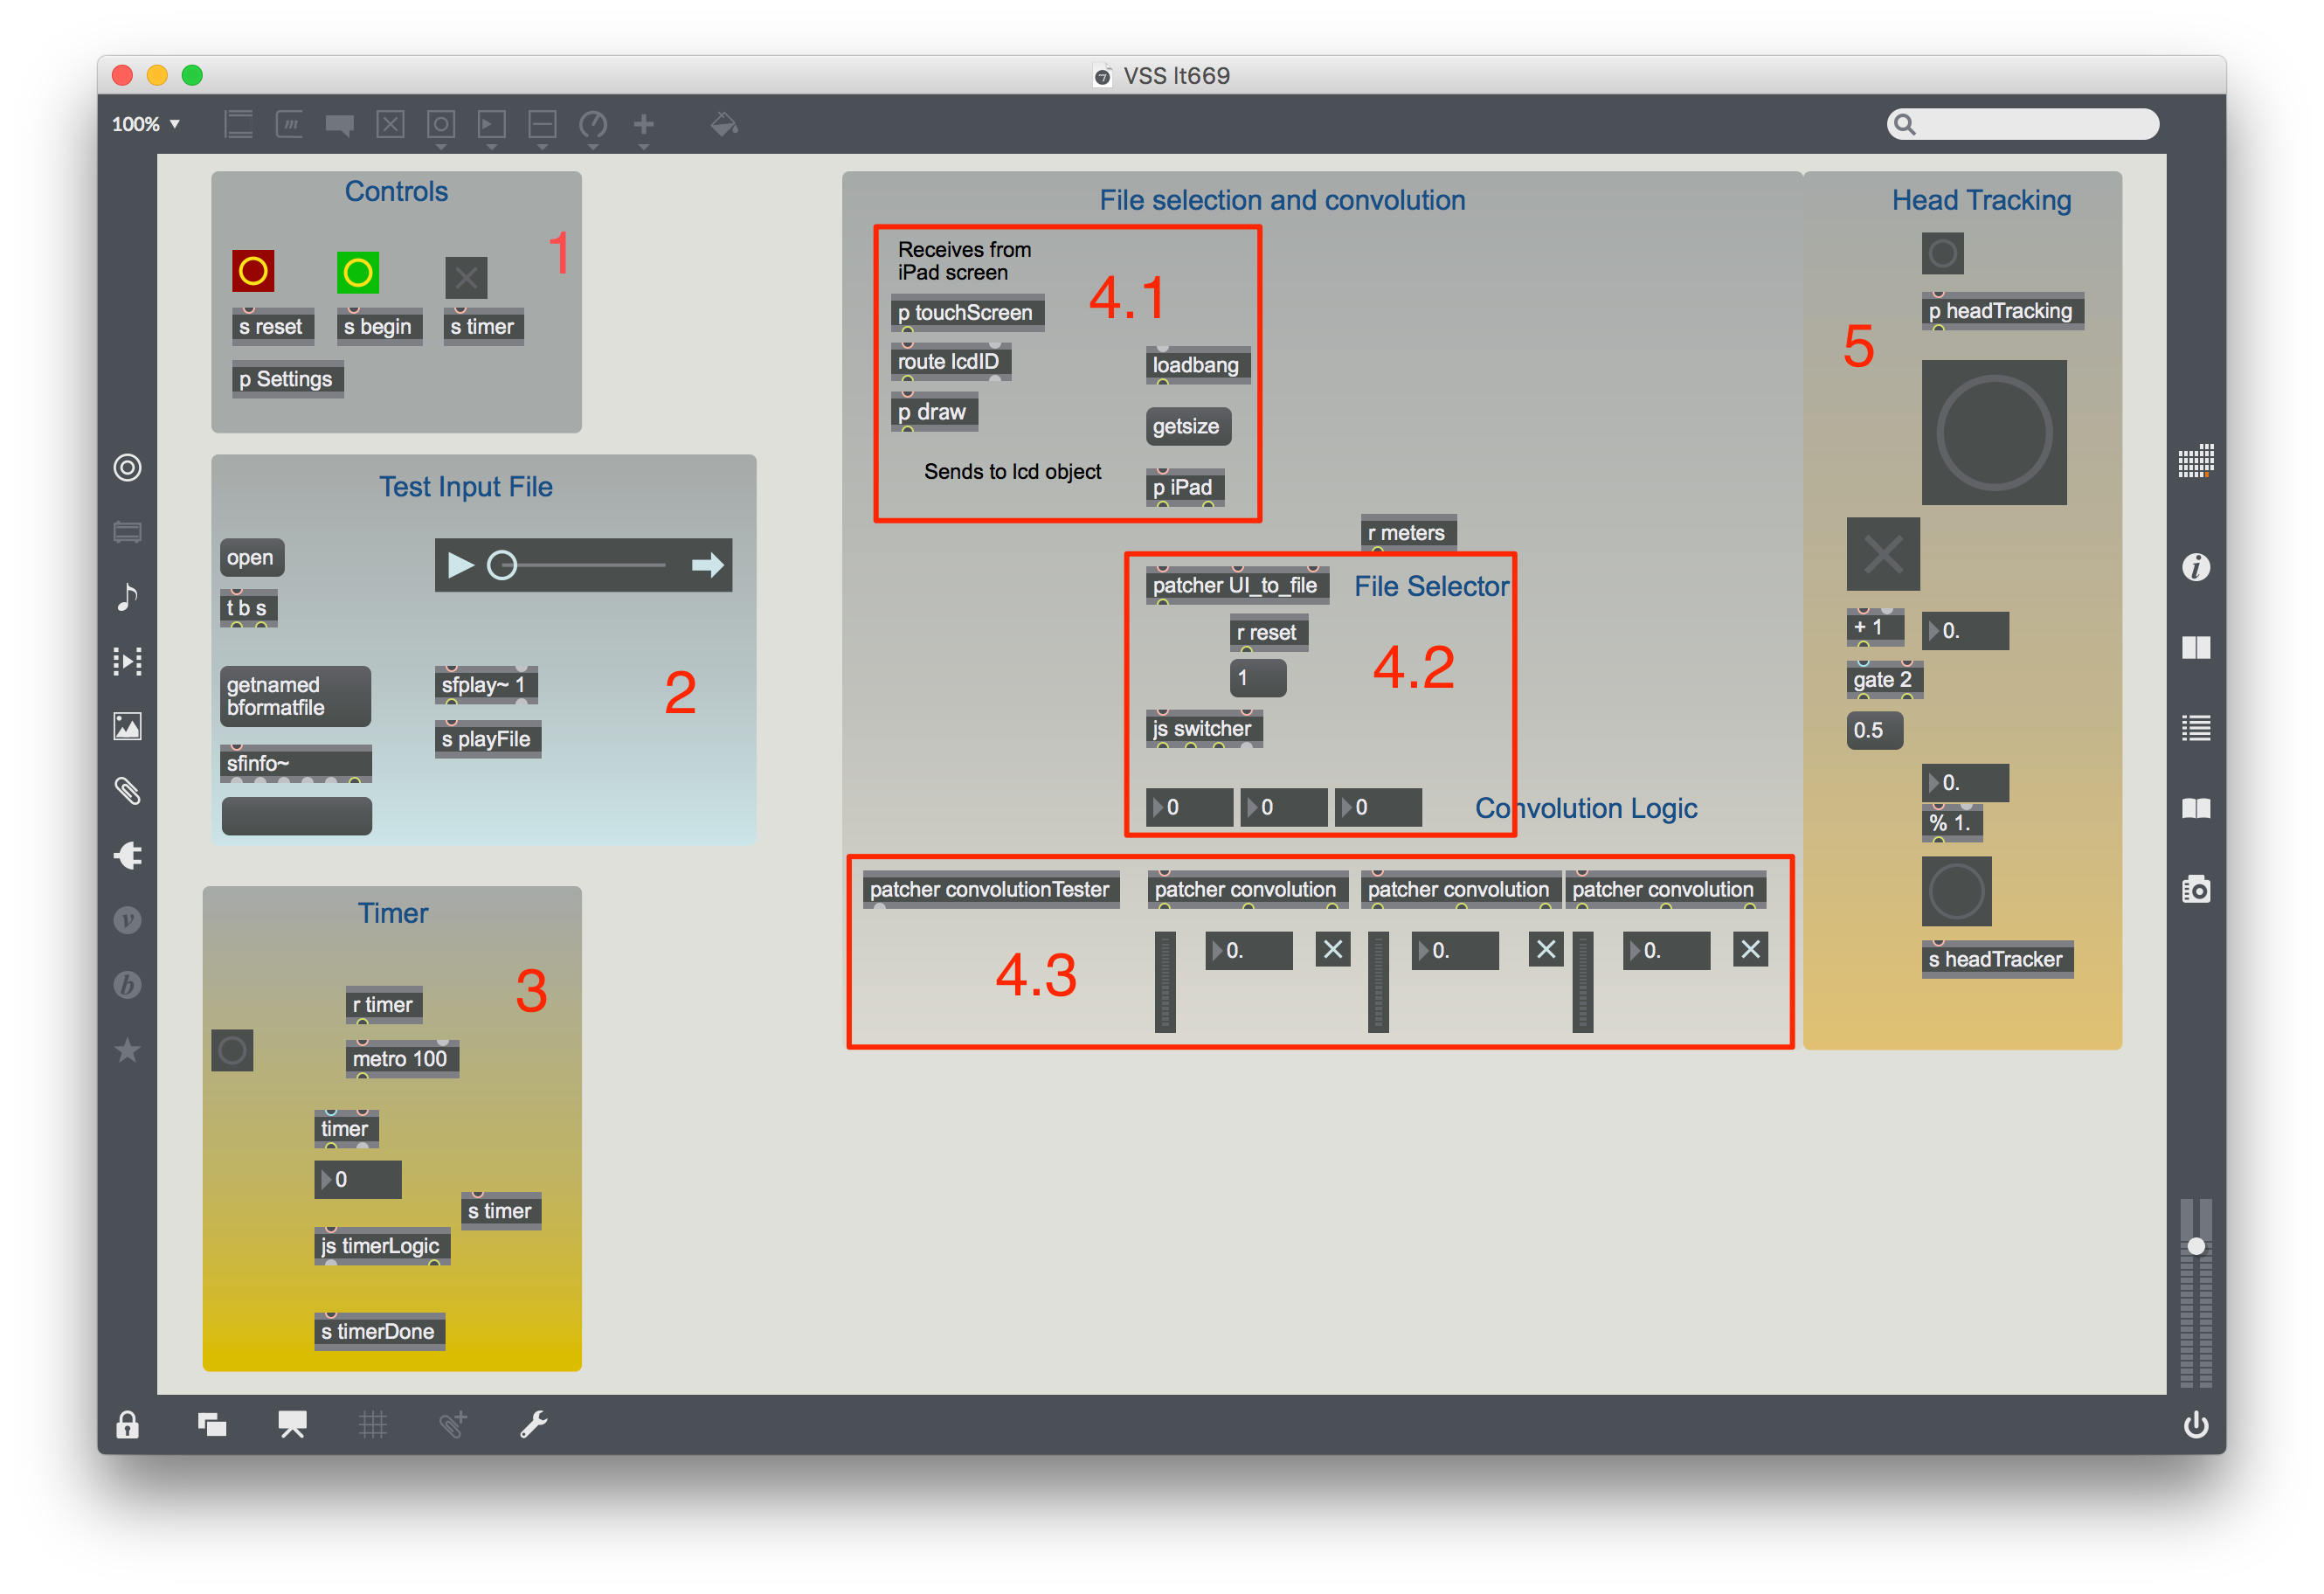
\includegraphics[scale = 0.4]{Sections/Implementation/Max/images/Max/MyPatch_Edit.png}}
					\caption{Top level Max patch}
					\label{myPatch}
				\end{figure}

		

				The software implementation was split into two main sections: \textbf{Location Selection} consisting of section \textbf{4.2} and \textbf{Mobility} mainly consisting of section \textbf{3 and 4.3}.



		\subsubsection{Location Selection}
			%User interface section
			%The location selection part of the system was required to present the user with an interface with which they could select a location within the \ac{VAE}. The system would then interpret their input and select the correct \ac{RIR} file(s) to be used in the rest of the system. 

			In order to allow the user to move themselves around the room, they had to be presented with a means of doing so. This involved presenting the user with an interface that resembled the space available to them on which they could select their location. This then had to output the coordinates selected by the user and convert them into a format which can be interpreted as a file name indicating which \ac{RIR} in the available grid to use. This could then be passed to the rest of the system to load the appropriate files. A simple block diagram of the user interface part of the system is shown in figure~\ref{flowDiagram}.


			%-------------Max UI Flow diagram-------------%
			\begin{figure}[H]
				\centerline{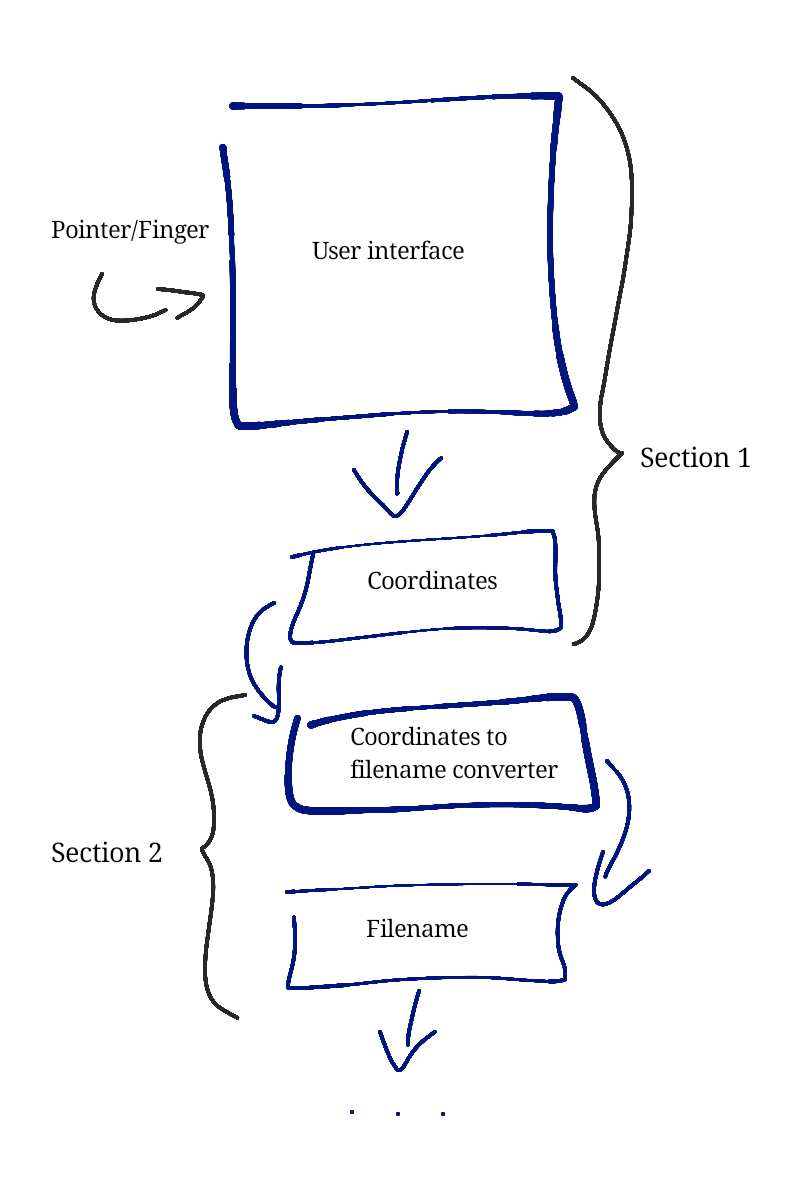
\includegraphics[scale = 0.3]{Sections/Implementation/Max/images/FlowDiagrams/Max1_V2.png}}
				\caption{Flow diagram of the location selection software design. \textbf{Section 1} indicates the user interface section where coordinates are recorded and \textbf{Section 2} takes these coordinates and finds the appropriate \ac{RIR} file.}
				\label{flowDiagram}
			\end{figure}

			In Max, the ‘lcd’ object is used for this function. This object presents a quadrilateral of variable length and height with the ability to output its dimensional information by sending a ‘getSize’ message to its input, as well as output the coordinates of a mouse click/drag. Figure~\ref{lcd} shows the lcd object with its inputs and outputs represented by section 1 in figure~\ref{flowDiagram}.

			%-------------LCD Image-------------%
			\begin{figure}[H]
				\centerline{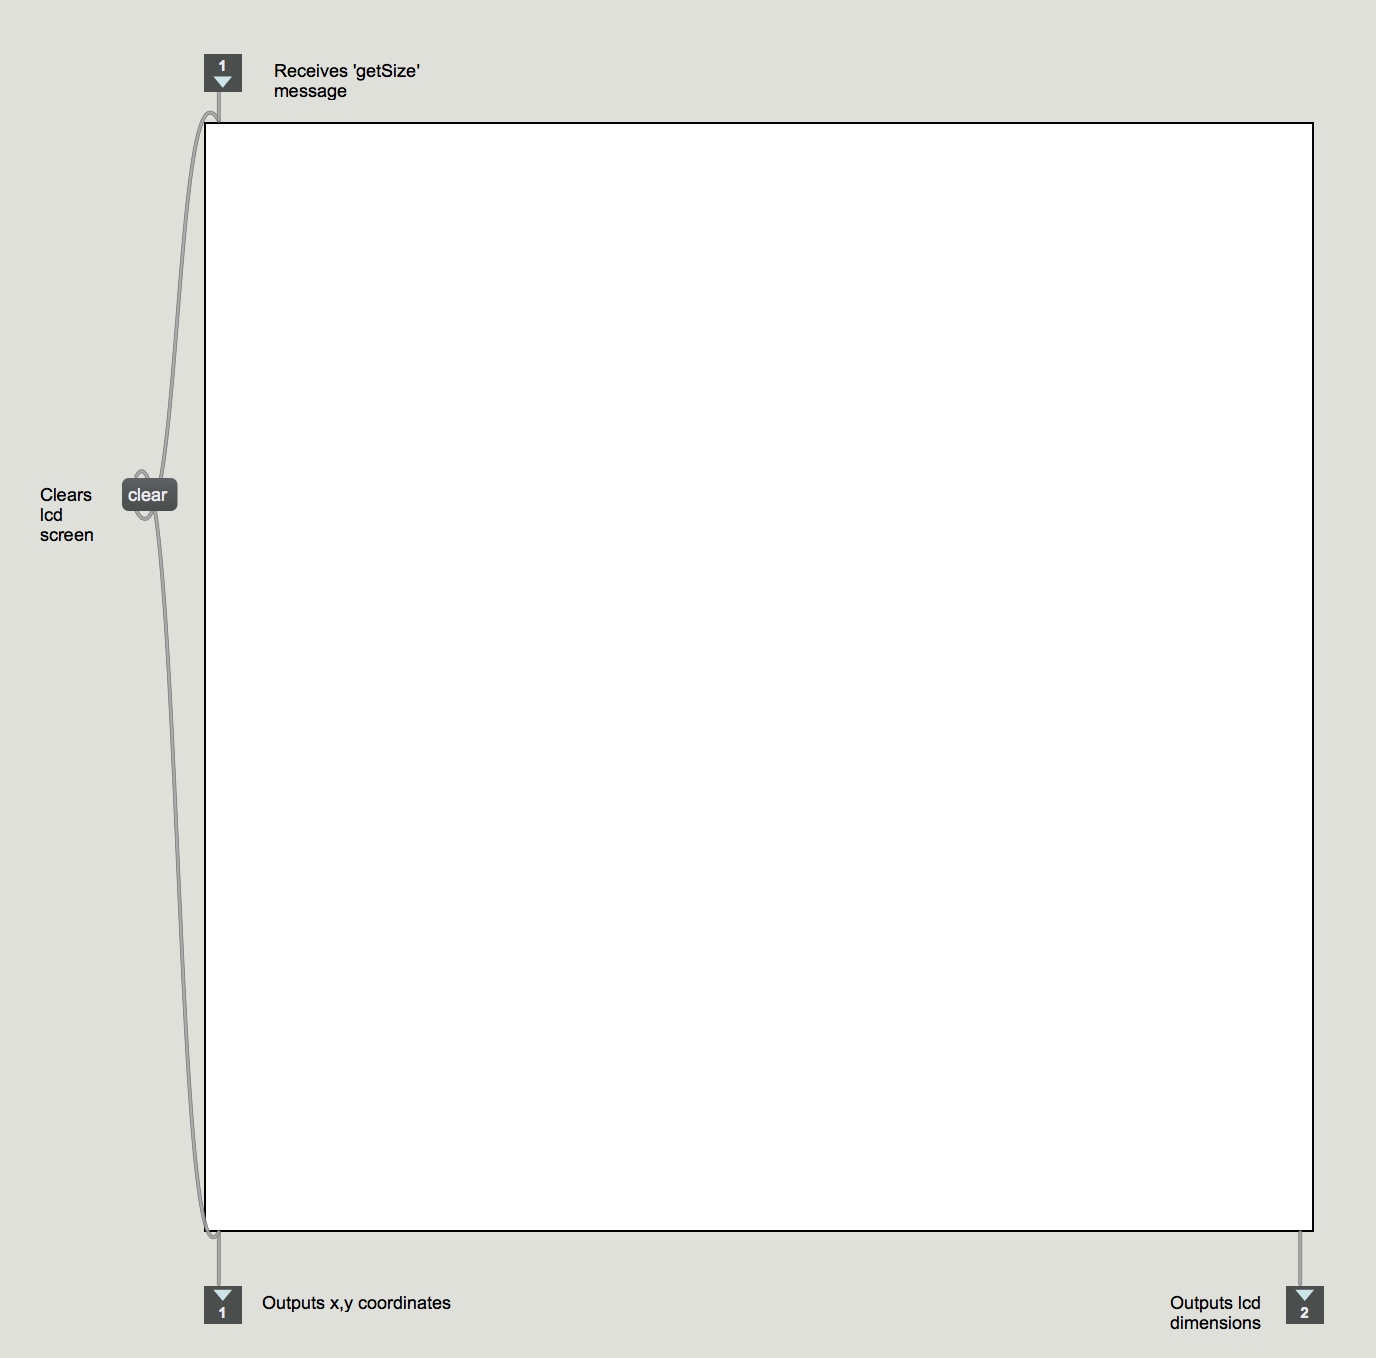
\includegraphics[scale = 0.4]{Sections/Implementation/Max/images/Max/lcd.png}}
				\caption{Flow diagram of the location selection software design}
				\label{lcd}
			\end{figure}

			The outputs from the lcd object are sent to the patch ‘UI\_to\_file’ which contains a JavaScript file called ‘loadFilesLogic’. This JavaScript file converts the (x,y) coordinates into an appropriate filename, by taking into account the size of the lcd screen and how many RIRs there are per meter.

			The javascript takes 5 inputs: UI (x,y) coordinates , (x,y) lcd dimensions and a number representing how many sections the lcd grid should be split into. This last value is calculated by sending a number from 1-5 (distance per RIR) to the third inlet of the UI\_to\_file patch (on the far right). As the maximum number of RIRs that will be available per length of the room is 15, the input is divided by 15 and rounded to the nearest value, giving the number of sections the lcd screen should be split into along the x-axis (the number of y-axis sections is calculated later). This information can then be used to determine in which \textit{‘section’} the user is currently located based on their coordinates, allowing it to load the appropriate RIRs that are available in that section. Figure~\ref{locationsConvert} shows the section of `UI\_to\_file' highlighting each section.

			%-------------UI_to_file Image-------------%
			\begin{figure}[H]
				\centerline{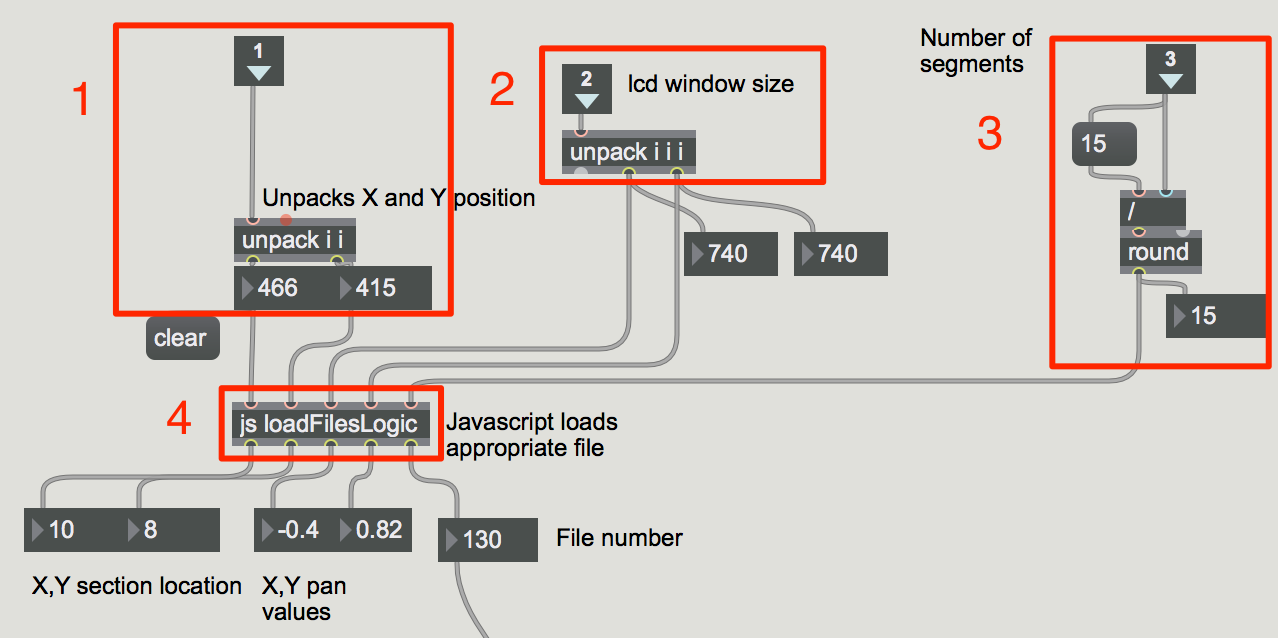
\includegraphics[scale = 0.6]{Sections/Implementation/Max/images/Max/UI_to_file_edit_3.png}}
				\caption{Screen shot from Max showing a section that converts the user interface coordinates into the appropriate file name. 1) Coordinates from lcd object 2) Dimensions of lcd object 3) Number of segments the lcd object should be split into due to the number of \ac{RIR}'s per meter 4) JavaScript file take produces an appropriate file name given the input data.}
				\label{locationsConvert}
			\end{figure}

			\paragraph{File name JavaScript: `loadFilesLogic'}

			%	\begin{wrapfigure}{R}{0.6\textwidth}
			\begin{minipage}{0.6\textwidth}
				\begin{lstlisting}
				function msg_int(input){
					if(inlet == 0){
						xPos = input; 
					} else if (inlet == 1){
						yPos = input;//Add off set to start at (0,1)
					} else if (inlet == 2){
						windowSize [0] = input;
					} else if (inlet == 3){
						windowSize [1] = input;
					} else if(inlet==4){
						numberOfMeters = input;
					}
				\end{lstlisting}
				\end{minipage}
				\begin{minipage}{0.35\textwidth}
				The first section in the JavaScript files simply stores the data from different inputs to different variables that are used throughout the rest of the code.
				\end{minipage}

				The code in figure~\ref{code2} calculates which section the user is closest to. The numberOfMeters variable is the 5th input to the js object which can be used to determine how many rows and columns of RIRs there are going to be. When the RIRs are separated by 3m or 5m, there are the same number of rows as there is columns (3m: 5x5) (5m: 3x3), whereas (1m: 15x16) the other distances produce grids of RIRs with one more row than there are columns. The if statement from 31 - 39 ensures that the lcd screen is split into the correct amount of sections in order to correctly load the appropriate RIR.

				\begin{figure}
				\begin{lstlisting}
					//Split into sections
					if(numberOfMeters == 3 || numberOfMeters == 5){
						//Even grid for 3m and 5m
						xPosition = (xPos/windowSize[0])*(numberOfMeters);
						yPosition = (yPos/windowSize[1])*(numberOfMeters);
					} else if (numberOfMeters == 4 || numberOfMeters == 8){
						//4m separation requires different x,y coordinate scaling
						xPosition = (xPos/windowSize[0])*(numberOfMeters-1);
						yPosition = (yPos/windowSize[1])*(numberOfMeters);
					} else{
						//Extra row for others
						xPosition = (xPos/windowSize[0])*(numberOfMeters); 
						yPosition = (yPos/windowSize[1])*(numberOfMeters+1);
					}	
					\end{lstlisting}
					\caption{Code}
					\label{code2}
					\end{figure}
				
					MMMMMMMBITCH
				

					\begin{lstlisting}
					//Round to nearest value
					xSection = Math.round(xPosition);
					ySection = Math.round(yPosition); 
					
					//Start the lcd grid sections from column 1 row 1 instead of column 0 row 0
					if(xSection == 0){
						xSection = 1; 
					}
					if(ySection == 0){
						ySection = 1;
					}
				\end{lstlisting}


	

		\subsubsection{Mobility Implementation}

		 \paragraph{Iteration 1}
		 	%Idea to stay between RIRs in a grid

		 	%Loading issued

		 \paragraph{Iteration 2}
		 	%Preload RIRs

		 \paragraph{Iteration 3}
		 \label{iteration3}
		 	%Path defining



	\subsection{Head-Tracking}
		YEI Sensor was not good.


	\subsection{Latency Test}
	
	\subsection{RIR Trimming}

\end{document}